% makeindex < aebpro_man.idx > aebpro_man.ind
\documentclass[12pt]{article}
\usepackage[fleqn]{amsmath}
\usepackage[
    web={centertitlepage,designv,forcolorpaper,latextoc,pro,addtoHyOpts={pagebackref=false}},
    eforms,
%    linktoattachments,
    aebxmp
]{aeb_pro}
\usepackage{richtext}
\usepackage{graphicx,array}
%\usepackage{myriadpro}
%\usepackage{calibri}
\usepackage[altbullet]{lucidbry}

%\previewtrue
%\usepackage{makeidx}
%\makeindex
\usepackage{acroman}
\usepackage[active]{srcltx}

\setcounter{secnumdepth}{4}
\setcounter{tocdepth}{5}
\makeatletter
\renewcommand*{\theparagraph}{\texorpdfstring{\protect\P\protect\ }{\textparagraph}}
\renewcommand{\paragraph}
    {\renewcommand{\@seccntformat}[1]{\theparagraph}%
    \@startsection{paragraph}{4}{0pt}{6pt}{-3pt}{\color{\aeb@subsubsectioncolor}\bfseries}}
\renewcommand*\l@paragraph{\@dottedtocline{4}{5.0em}{1em}} %{7.0em}{4.1em}}
\def\chgCurrLblName#1{\def\@currentlabelname{#1}}
\def\echgCurrLblName#1{\edef\@currentlabelname{#1}}
\makeatother

\getDimsFromGraphic{graphics/dpsweb}{\dpswebW}{\dpswebH}


%\urlstyle{rm}
\urlstyle{sf}
\let\uif\textsf
\let\app\textsf
\def\psf#1{\textbf{\textsf{#1}}}
\let\amtIndent\leftmargini

\convertcolorspec{named}{red}{RGB}{\rgbRed}
\convertcolorspec{named}{blue}{RGB}{\rgbBlue}
\convertcolorspec{named}{red}{HTML}{\htmlRed}
\convertcolorspec{named}{blue}{HTML}{\htmlBlue}
\convertcolorspec{named}{magenta}{RGB}{\rgbMagenta}
\convertcolorspec{named}{magenta}{HTML}{\htmlMagenta}
\convertcolorspec{named}{webbrown}{HTML}{\htmlWebBrown}

\renewcommand*\descriptionlabel[1]{\hspace\labelsep
    \normalfont #1}


\DeclareDocInfo
{
    university={Acro\negthinspace\TeX.Net},
    title={\textsf{richtext}: A method of creating rich text strings},
    author={D. P. Story},
    email={dpstory@acrotex.net},
    subject={Documentation for the richtext package from AcroTeX},
    talksite={\url{www.acrotex.net}},
    version={v1.0c, 2016/10/03},
    keywords={AcroTeX, rich text strings},
    copyrightStatus=True,
    copyrightNotice={Copyright (C) \the\year, D. P. Story},
    copyrightInfoURL={http://www.acrotex.net}
}

\def\dps{$\hbox{$\mathfrak D$\kern-.3em\hbox{$\mathfrak P$}%
   \kern-.6em \hbox{$\mathcal S$}}$}

\universityLayout{fontsize=Large}
\titleLayout{fontsize=LARGE}
\authorLayout{fontsize=Large}
\tocLayout{fontsize=Large,color=aeb}
\sectionLayout{indent=-62.5pt,fontsize=large,color=aeb}
\subsectionLayout{indent=-31.25pt,color=aeb}
\subsubsectionLayout{indent=0pt,color=aeb}
\subsubDefaultDing{\texorpdfstring{$\bullet$}{\textrm\textbullet}}

\widestNumber{0.00.}
%\pagestyle{empty}
%\parindent0pt\parskip\medskipamount

\def\dps{$\mbox{$\mathfrak D$\kern-.3em\mbox{$\mathfrak P$}%
   \kern-.6em \hbox{$\mathcal S$}}$}

\newcount\fldCnt \fldCnt=0
\def\incFldCnt{\global\advance\fldCnt1\relax}

\frenchspacing

\chngDocObjectTo{\newDO}{doc}
\begin{docassembly}
var titleOfManual="The AeB RichText MANUAL";
var manualfilename="Manual_BG_Print_richtext.pdf";
var manualtemplate="Manual_BG_Brown.pdf"; // Blue, Green, Brown
var _pathToBlank="C:/Users/Public/Documents/ManualBGs/"+manualtemplate;
var doc;
var buildIt=false;
if ( buildIt ) {
    console.println("Creating new " + manualfilename + " file.");
    doc = \appopenDoc({cPath: _pathToBlank, bHidden: true});
    var _path=this.path;
    var pos=_path.lastIndexOf("/");
    _path=_path.substring(0,pos)+"/"+manualfilename;
    \docSaveAs\newDO ({ cPath: _path });
    doc.closeDoc();
    doc = \appopenDoc({cPath: manualfilename, oDoc:this, bHidden: true});
    f=doc.getField("ManualTitle");
    f.value=titleOfManual;
    doc.flattenPages();
    \docSaveAs\newDO({ cPath: manualfilename });
    doc.closeDoc();
} else {
    console.println("Using the current "+manualfilename+" file.");
}
var _path=this.path;
var pos=_path.lastIndexOf("/");
_path=_path.substring(0,pos)+"/"+manualfilename;
\addWatermarkFromFile({
    bOnTop:false,
    bOnPrint:false,
    cDIPath:_path
});
\executeSave();
\end{docassembly}

\begin{document}

\maketitle

\selectColors{linkColor=black}
\tableofcontents
\selectColors{linkColor=webgreen}

\def\AcroT{Acro\!\TeX}\def\cAcroT{\textcolor{blue}{\AcroT}}
\def\AcroEB{\AcroT{} eDucation Bundle}\def\cAcroEB{\textcolor{blue}{\AcroEB}}
\def\AcroB{\AcroT{} Bundle}\def\cAcroB{\textcolor{blue}{\AcroB}}
\def\bUrl{http://www.math.uakron.edu/~dpstory}

\hypersetup{linktocpage}


%FreeText
%/C[1.0 1.0 1.0]/Contents(This is test If there a real test, we would all be in trouble.)
%/CreationDate(D:20160909063701-05'00')
%/DA(0.898 0.1333 0.2157 rg /Helv 12 Tf)
%/DS(font: Helvetica,sans-serif 12.0pt; text-align:left; color:#E52237 )
%/F 4/M(D:20160909065147-05'00')/NM(f8e9e6b1-1651-4c47-9169-8a47c7af23ff)
%/RC(<?xml version="1.0"?><body xmlns="http://www.w3.org/1999/xhtml" xmlns:xfa="http://www.xfa.org/schema/xfa-data/1.0/" xfa:APIVersion="Acrobat:15.19.0" xfa:spec="2.0.2"  style="font-size:12.0pt;text-align:left;color:#E52136;font-weight:normal;font-style:normal;font-family:Helvetica,sans-serif;font-stretch:normal">
%<p dir="ltr">
%<span style="text-align:justify;color:#FF0000;font-family:Helvetica">
%    This is </span>
%<span style="text-decoration:line-through;text-align:justify;color:#FF0000;font-weight:bold;font-style:italic;font-family:Helvetica">
%    test</span>
%<span style="text-align:justify;color:#FF0000;font-family:Helvetica">
%If there a real test, we would all be in trouble.</span>
%</p></body>)/Rect[30.1092 174.763 181.964 251.345]/Subj(Text Box)/Subtype/FreeText/T(dpstory)/Type/Annot>>


\section{Introduction}

Rich text contents for variable text (text fields and editable combo boxes)
and markup annotations was introduced into the PDF specification beginning
with PDF 1.5 (\app{Acrobat} and \app{Adobe Reader} version~6). The rich text
strings are difficult to create for it requires reading from a number of
sources. The \pkg{richtext} package provides commands and documentation
needed to ``easily'' produce such rich strings. We demonstrate the results
using the \pkg{eforms} package (the text field produced by \pkg{hyperref}
does not support rich text).

References for this material includes the \textsl{PDF
Reference}~\cite{book:pdfspec}, the XFA specification~\cite{webpage:XFASpec},
and the CSS2 specification~\cite{webpage:CSS2}. Additionally, the \textsl{JavaScript for
Acrobat API Reference}~\cite{tech:AcroJS} covers the JavaScript API for
handling rich text content.

\section{Preamble: Required packages and options}

The package has no options and only requires \pkg{xkeyval} and \pkg{ifxetex} packages.
The package can produce rich text strings, but to actually use them, you'll need
the \pkg{eforms} package.

The package works for all drivers \app{dvips}, \app{pdflatex}, \app{xelatex},
and \app{luatex}. The \pkg{eforms} package can automatically detect all
drivers except \pkg{dvips}, and that is used by default.

\section{Creating rich text strings}\label{s:CreateRTS}

We begin by illustrating the result of the \pkg{richtext} package, consider the rich text field below.

\rtpara[indent=first]{para1}{Now is the time for
\span{style={bold,italic,strikeit},color=ff0000}{J\374rgen} and all
good men to come to the aid of \it{their} \bf{country}. Now is the time for
\span{style=italic}{all good} women to do the same.}
\rtpara[indent=first]{para2}{With rich text, we can format the text within
the text field. As a reader of this rich text field, you can edit the
contents of the box, feel free to do so.}
\rtpara[halign=right]{para3}{D. P. Story \span{url=http://www.acrotex.net}{AcroTeX.Net}}

\setRVVContent{myContent}{{para1}{para2}{skipline}{para3}}

\begin{center}
%\previewtrue
\incFldCnt
\textField[\Ff{\FfRichText}\Ff{\FfMultiline}
\DS{\useDefaultDS}%\DS{\useDS{myDS}}%
\RV{\useRVContent{myContent}}\V{\useVContent{myContent}}]{rtFld\the\fldCnt}{4in}{10\baselineskip}
\end{center}

To edit the field above, click in the field, press \uif{Ctrl+E} or \uif{Cmd+E} (for \app{Mac OS}) to obtain
the \uif{Form Field Text Properties} toolbar. By pressing the \uif{More} button, you can see the additional
properties of the field, as seen in \hyperref[fig:FPtabs]{Figure~\ref*{fig:FPtabs}}.


A rich text may have any of several style attributes, many of these are illustrated in the above example.
As a guide to introducing the attributes, we follow the \uif{Form Field Text Properties} dialog box shown
in \hyperref[fig:FPtabs]{Figure~\ref*{fig:FPtabs}}.

\begin{figure}[htb]\centering\setlength{\fboxsep}{0pt}%
\fbox{\parbox{.5\linewidth-5pt-2\fboxrule}{\includegraphics[width=\linewidth]{graphics/fontprops}}}\hspace{10pt}%
\fbox{\parbox{.5\linewidth-5pt-2\fboxrule}{\includegraphics[width=\linewidth]{graphics/paragraphprops}}}\\[6pt]
\fbox{\parbox{.8\linewidth-2\fboxrule}{\includegraphics[width=\linewidth]{graphics/linkprops}}}%
\caption{The Font, Paragraph and Link tabs}\label{fig:FPtabs}
\end{figure}

\newtopic\noindent
The basic command for creating a rich text \emph{paragraph} is \cs{rtpara}:
\bVerb\takeMeasure{\string\rtpara[\ameta{Para-Font-attrs}]\darg{\ameta{name}}\darg{\ameta{rich-text-paragraph}}}%
\begin{dCmd}[commandchars=!()]{\bxSize}
\rtpara[!ameta(Para-Font-attrs)]{!ameta(name)}{!ameta(rich-text-paragraph)}
\end{dCmd}
\eVerb where \ameta{Para-Font-attrs} are key-value pairs (in the {\LaTeX}
sense) that are described in \hyperref[s:FLtabs]{Sections~\ref*{s:FLtabs}}
and~\ref{s:Paratab}; these attributes are applied to the paragraph as a
whole. The \ameta{name} is a unique name to be associated with
\ameta{rich-text-paragraph} so it can be referenced later from within a text
field. There are two types of attributes: \uif{Font} and \uif{Paragraph}, as
guided by \hyperref[fig:FPtabs]{Figure~\ref*{fig:FPtabs}}. For convenience,
the \uif{Link} attributes (URLs) are classified as \uif{Font}. The optional
argument of \cs{rtpara} consists of usually \uif{Paragraph} attributes, most
\uif{Font} attributes are also recognized.

The definition of the first paragraph of the above rich text field reads as
follows:
\begin{Verbatim}[fontsize=\small]
\rtpara[indent=first]{para1}{Now is the time for
    \span{style={bold,italic,strikeit},color=ff0000}{J\374rgen}
    and all good men to come to the aid of \it{their}
    \bf{country}. Now is the time for \span{style=italic}
    {all good} women to do the same.}
\end{Verbatim}
In this example, the optional argument for \cs{rtpara} was used to indent the
paragraph. The rich text defined here is named \texttt{para1}. The third
argument, \ameta{rich-text-string}, consists of ordinary text, the \cs{span}
command used to insert special formatting for text, and certain other
`short-cut' markups like \cs{it} and \cs{bf}. Note that the umluat (\"{u}) is
expressed as octal (\cs{374}).

The \cs{span} command is used to format individual sentence fragments. Its
syntax is,
\bVerb\takeMeasure{\string\span\darg{\ameta{Font-attrs}}\darg{\ameta{rich-text-string}}}%
\begin{dCmd}[commandchars=!()]{\bxSize}
\span[!ameta(Font-attrs)]{!ameta(rich-text-string)}
\end{dCmd}
\eVerb where \ameta{Font-attrs} are \uif{Font} attributes as described in
\hyperref[s:FLtabs]{Sections~\ref*{s:FLtabs}}; these attributes are applied
to the string \ameta{rich-text-string} only. The \cs{span} command, as
described here, is only defined within the third argument
(\ameta{rich-text-paragraph}) of \cs{rtpara}. This is necessary because
\cs{span} is a {\TeX} primitive command, and we must not overwrite its
definition.

When you create a \emph{rich text string} there is a parallel development of a
\emph{plain text string}, the string without its rich text markup, these two
(rich and plain strings) are used to populate the values of the \psf{RV} and
\psf{V} keys of a text field. When you define a rich text paragraph string
under its own \ameta{name}, you can typeset it (to check the syntax) and its
plain text counterpart using the \cs{useRV\darg{\ameta{name}}} and
\cs{useV\darg{\ameta{name}}} commands. For example,
\begin{quote}\raggedright\ttfamily\makeatletter\def\rt@SC{;\penalty0}%
\rtpara[indent=first]{para1}{Now is the time for
\span{style={bold,italic,strikeit},color=ff0000}{J\string\374rgen} and all
good men to come to the aid of \it{their} \bf{country}. Now is the time for
\span{style=italic}{all good} women to do the same.}
\makeatother
\hspace*{-\leftmargini}\textbf{\cs{useRV\darg{para1}:}}\ \useRV{para1}\\[\baselineskip]
\hspace*{-\leftmargini}\textbf{\cs{useV\darg{para1}:}}\ \useV{para1}
\end{quote}
These commands may also be used to insert the strings into the \psf{RV} and
\psf{V} keys, respectively; though the \pkg{richtext} package offers an
alternative technique.

\subsection{The \texorpdfstring{\uif{Font}}{Font} and
\texorpdfstring{\uif{Link}}{Link} tabs}\label{s:FLtabs}

In this section, we cover the \uif{Font} and \uif{Link} tabs, as well as other attributes
not listed on any tab.

\subsubsection{The \texorpdfstring{\uif{Font}}{Font} tab}

We discuss the \uif{Font} tab of \hyperref[fig:FPtabs]{Figure~\ref*{fig:FPtabs}}. The
key-value for each of the attributes is given and described briefly. These key-values
may appear as \ameta{Font-attrs} or \ameta{Para-Font-attrs}.
\begin{description}
%The font family used to draw the text. It is an array of family names to be searched for in order. The first
%entry in the array is the font name of the font to use. The second entry is an optional generic family name
%to use if an exact match of the first font is not found. The generic family names are
%symbol, serif, sans-serif, cursive, monospace, fantasy
%The default generic family name is sans-serif.
\item[\uif{Font:}] \texttt{font=\ameta{font\_name}} A font name or a list of
    font names to be used to display the enclosed text. The first
    entry is the font name of the font to use. The second font name is
    typically a generic family name to use if an exact match is not found.
    The generic family names are \texttt{symbol}, \texttt{serif},
    \texttt{sans-serif}, \texttt{cursive}, \texttt{monospace}, and
    \texttt{fantasy}. The default is \texttt{sans-serif}. If a typeface name
    contains white space, enclose it within single quotes (\texttt{'}).
\begin{flushleft}\small %\previewtrue
\verb|\rtpara[font={Arial,sans-serif}]{para1}{This is Arial or a|
\hspace*{20pt}\verb|san-serif substitute.}|\\[3pt]
\rtpara[font={Arial,sans-serif}]{para1}{This is Arial or a san-serif substitute.}%
\incFldCnt\textField[\Ff{\FfRichText}%\Ff{\FfMultiline}
\DS{\useDefaultDS}\RV{\useRV{para1}}\V{\useV{para1}}]{rtFld\the\fldCnt}{3in}{16bp}\\[6pt]
\verb|\rtpara{para2}{This is \span{font='Myriad Pro'}|
\hspace*{20pt}\verb|{Myriad Pro} font.}|\\[3pt]
\rtpara{para2}{This is \span{font='Myriad Pro'}{Myriad Pro} font.}
\incFldCnt\textField[\Ff{\FfRichText}%\Ff{\FfMultiline}
\DS{\useDefaultDS}\RV{\useRV{para2}}\V{\useV{para2}}]{rtFld\the\fldCnt}{3in}{16bp}
\end{flushleft}
In the second example, only `Myriad Pro' is actually set in the Myriad Pro font; the rest of the sentence
is typeset in the default font, Helvetica in this case. Use \uif{Ctrl+E} (\uif{Cmd+E}) to inspect the properties
of these two fields and verify the fonts are Arial, Myriad Pro, and Helvetica.

\item[\uif{Size}:] \texttt{size=\ameta{dec\_num}} The size of the font to
    be used. The value of \texttt{size} is \ameta{dec\_num}, a (positive)
    decimal number.
\begin{flushleft}\small %\previewtrue
\verb|\rtpara[size=12]{para1}{This is 12pt font, while|
\hspace*{20pt}\verb|\span{size=8}{this is 8pt font.} OK?}|\\[6pt]
\rtpara[size=12]{para1}{This is 12pt font, while \span{size=8}{this is 8pt font.} OK?}
\incFldCnt\textField[\Ff{\FfRichText}%\Ff{\FfMultiline}
\DS{\useDefaultDS}\RV{\useRV{para1}}\V{\useV{para1}}]{rtFld\the\fldCnt}{3in}{16bp}
\end{flushleft}

\item[\uif{Baseline Shift:}] \texttt{raise=\ameta{def\_num}} The position of the baseline of the text is determined
by the \texttt{raise} key. \texttt{raise=6.6} raises the baseline \texttt{6.6pt}, while \texttt{raise=-4} lowers
it \texttt{4pt}.
\begin{flushleft}\small
\verb|\rtpara{para1}{This text \span{raise=6.6}{is raised by|
\hspace*{20pt}\verb| 6.6pt} while this text \span{raise=-4}|
\hspace*{20pt}\verb|{is lowed by 4pt.} Back to normal baselines.}|\\[6pt]
\rtpara{para1}{This text \span{raise=6.6}{is raised by 6.6pt} while this text
\span{raise=-4}{is lowed by 4pt.} Back to normal baselines.}
\incFldCnt\textField[\Ff{\FfRichText}\Ff{\FfMultiline}
\DS{\useDefaultDS}\RV{\useRV{para1}}\V{\useV{para1}}]{rtFld\the\fldCnt}{3in}{16bp*4}
\end{flushleft}

\item[\uif{Underline:}]
    \texttt{ulstyle=\ameta{\upshape{none|ul|2ul|wul|2wul}}} The
    \texttt{ulstyle} key determines the style of underlining, possible values
    are \texttt{none} (no underlining), \texttt{ul} (underlining),
    \texttt{2ul} (double-line underlining), \texttt{wul} (word underlining),
    and \texttt{2wul} (double-line word underlining).
\begin{flushleft}\small %\previewtrue
\verb|\rtpara{para1}{We can \span{ulstyle=ul}{underline in a}|
\hspace*{20pt}\verb|\span{ulstyle=2ul}{number of different ways}|
\hspace*{20pt}\verb|\span{ulstyle=wul}{that catch the}|
\hspace*{20pt}\verb|\span{ulstyle=2wul}{attention of the reader}.|\\[3pt]
\rtpara{para1}{We can \span{ulstyle=ul}{underline in a} \span{ulstyle=2ul}{number of different ways}
\span{ulstyle=wul}{that catch the} \span{ulstyle=2wul}{attention of the reader}.}
\incFldCnt\textField[\Ff{\FfRichText}\Ff{\FfMultiline}
\DS{\useDefaultDS}\RV{\useRV{para1}}\V{\useV{para1}}]{rtFld\the\fldCnt}{3in}{16bp*4}
\end{flushleft}

\item[\uif{Style}:]
    \texttt{style=\darg{\upshape{[bold,][italic,][strikeit]}}} Unlike some
    of the other (choice) keys, the value of the \texttt{style} key is any
    \emph{subset} of the values listed:  for example, \texttt{style=bold}
    paints the underlying text in bold, \texttt{style=\darg{bold,italic}}
    yields bold-italic font, and, for a final example,
    \texttt{style=\darg{italic,strikeit}} typesets its text in
    strike-through italic. Multiple values must be enclosed in braces
    (\darg{}) so that \pkg{xkeyval} can correctly parse them.
\begin{flushleft}\small %\previewtrue
\verb|\rtpara{para1}{To \span{style=bold}{boldly to go} where|
\hspace*{20pt}\verb|\span{style={bold,italic}}{no man has gone}|
\hspace*{20pt}\verb|\span{style={italic,strikeit}}{prior}|
\hspace*{20pt}\verb|\span{style={italic,bold}}{before.}|\\[3pt]
\rtpara{para1}{To \span{style=bold}{boldly to go} where
\span{style={bold,italic}}{no man has gone}
\span{style={italic,strikeit}}{prior}\span{style={italic,bold}}{before.}}
\incFldCnt\textField[\Ff{\FfRichText}\Ff{\FfMultiline}
\DS{\useDefaultDS}\RV{\useRV{para1}}\V{\useV{para1}}]{rtFld\the\fldCnt}{3in}{16bp*2}
\end{flushleft}

\item[\uif{Color:}]
    \texttt{color=\ameta{\upshape{\meta{rrggbb}|\darg{rgb(\meta{rrr,ggg,bbb})}}}}
    Use this key to color the effected text. There are two
    methods of defining color:
\begin{itemize}
    \item[(1)] \meta{rrggbb} uses a 2-digit hexadecimal
    value for each component;
    \item[(2)] \texttt{rgb(\meta{rrr,ggg,bbb})} uses a decimal
    value (0--255) for each component.
\end{itemize}
    Because the second form contains
    commas, it must necessarily be enclosed in braces (\darg{}) to be
    correctly parsed by \pkg{xkeyval}.
\begin{flushleft}\small %\previewtrue
\verb|\rtpara{para1}{This is \span{color={rgb(255,0,0)}}{red} and|
\hspace*{20pt}\verb|this is \span{color=0000ff}{blue}.|
\rtpara{para1}{This is \span{color={rgb(255,0,0)}}{red} and this is \span{color=0000ff}{blue}.}\\[3pt]
\incFldCnt\textField[\Ff{\FfRichText}%\Ff{\FfMultiline}
\DS{\useDefaultDS}\RV{\useRV{para1}}\V{\useV{para1}}]{rtFld\the\fldCnt}{3in}{16bp}
\end{flushleft}
Things are not as bad as it seems. The \pkg{xcolor} package has the
wonderful command \cs{convertcolorspec} that converts colors between color
models. For example, we might define:
\begin{Verbatim}[fontsize=\small]
\convertcolorspec{named}{red}{RGB}{\rgbRed}
\convertcolorspec{named}{blue}{HTML}{\htmlBlue}
\convertcolorspec{named}{magenta}{RGB}{\rgbMagenta}
\convertcolorspec{named}{magenta}{HTML}{\htmlMagenta}
\end{Verbatim}
We can then use these named colors.
\begin{Verbatim}[fontsize=\small]
\rtpara{para1}{This is \span{color={rgb(\rgbRed)}}{red} and
this is \span{color=\htmlBlue}{blue}. We can do magenta two
ways, using \span{color={rgb(\rgbMagenta)}}{decimal
components} or using \span{color=\htmlMagenta}{hexadecimal
components}.}
\end{Verbatim}
\rtpara{para1}{This is \span{color={rgb(\rgbRed)}}{red} and this
is \span{color=\htmlBlue}{blue}. We can do magenta two ways,
using \span{color={rgb(\rgbMagenta)}}{decimal components} or
using \span{color=\htmlMagenta}{hexadecimal components}.}\par\smallskip
\incFldCnt\textField[\Ff{\FfRichText}\Ff{\FfMultiline}
\DS{\useDefaultDS}\RV{\useRV{para1}}\V{\useV{para1}}]{rtFld\the\fldCnt}{3in}{16bp*4}\\[6pt]
%
Notice that \verb|color={rgb(\rgbMagenta)}|, the value of \texttt{color}, is
still enclosed in braces since the expansion of \cs{rgbMagenta} contains
commas.
\end{description}

\subsubsection{The \texorpdfstring{\uif{Link}}{Link} tab}

We can create a link within rich text by using the \texttt{url} key from within
the first argument of the \cs{span} command. The syntax is \texttt{url=\ameta{URL}}.
\begin{Verbatim}[fontsize=\small]
\rtpara{para1}{Visit me at \span{url={http://www.acrotex.net},
    font='Courier New'}{http://www.acrotex.net}}
\end{Verbatim}
\begin{quote}
\rtpara{para1}{Visit me at \span{url={http://www.acrotex.net},font='Courier New'}{http://www.acrotex.net}}\par\smallskip
\incFldCnt\textField[\Ff{\FfRichText}%\Ff{\FfMultiline}
\DS{\useDefaultDS}\RV{\useRV{para1}}\V{\useV{para1}}]{rtFld\the\fldCnt}{3.5in}{16bp}
\end{quote}
It appears the \app{Acrobat/Reader} applications format a URL in underlined blue. We can override this however.
\begin{Verbatim}[fontsize=\small]
\rtpara{para1}{Visit me at \span{url={http://www.acrotex.net},
    color=\htmlMagenta,ulstyle=none,font='Courier New'}
    {http://www.acrotex.net}}
\end{Verbatim}
\begin{quote}
\rtpara{para1}{Visit me at \span{url={http://www.acrotex.net},
    color=\htmlMagenta,ulstyle=none,font='Courier New'}
    {http://www.acrotex.net}}
\par\smallskip
\incFldCnt\textField[\Ff{\FfRichText}%\Ff{\FfMultiline}
\DS{\useDefaultDS}\RV{\useRV{para1}}\V{\useV{para1}}]{rtFld\the\fldCnt}{3.5in}{16bp}
\end{quote}
Special characters are no problem, with the exception of wrapping a long URL
around to a different line (usually needed for display purposes):
\begin{Verbatim}[fontsize=\small]
\rtpara{para1}{Visit me at
    \span{url={http://www.math.uakron.edu/~dpstory/%
    acrotex.html#technical}}{AcroTeX at The University
    of Akron}}
\end{Verbatim}
\begin{quote}
\rtpara{para1}{Visit me at \span{url={http://www.math.uakron.edu/%
    ~dpstory/acrotex.html#technical}}
    {AcroTeX at The University of Akron}}\par\smallskip
\incFldCnt\textField[\Ff{\FfRichText}\Ff{\FfMultiline}
\DS{\useDefaultDS}\RV{\useRV{para1}}\V{\useV{para1}}]{rtFld\the\fldCnt}{3.5in}{16bp*2}
\end{quote}

\subsubsection{Miscellaneous markup of the \texorpdfstring{\uif{Font}}{Font} classification}

There are several other attributes that are not key-values, but are
implemented through {\LaTeX} commands.

\paragraph[Bold and italic]{Bold and italic.}\chgCurrLblName{Bold and italic}\label{para:BandI}
There are a couple of XHTML
elements that can also be used for bold and italic.
\begin{itemize}
    \item \cs{bf\darg{\ameta{text}}} expands to \texttt{<b>\ameta{text}</b>} and places
    \ameta{text} in bold font. May be used within a \cs{span} command.
    \item \cs{it\darg{\ameta{text}}} expands to \texttt{<i>\ameta{text}</i>} and places
    \ameta{text} in italic font. May be used within a \cs{span} command.
\end{itemize}
Both \cs{bf} and \cs{it} are local commands, undefined outside of the third argument
of \cs{rtpara}. Do  not code \texttt{<b>\ameta{text}</b>} or \texttt{<i>\ameta{text}</i>}
directly, rather, always use the {\LaTeX} commands \cs{bf} and \cs{it}. \cs{bf} and \cs{it} may be nested.
\begin{Verbatim}[fontsize=\small]
\rtpara{para1}{We \bf{boldly} say that \it{italic} is used for
emphasis, but both \bf{\it{drive home the point}}.}
\end{Verbatim}
\begin{quote}
\rtpara{para1}{We \bf{boldly} say that \it{italic} is used for emphasis,
but both \span{color=\htmlBlue}{\bf{\it{drive home the point}}}.}
\incFldCnt\textField[\Ff{\FfRichText}\Ff{\FfMultiline}
\DS{\useDefaultDS}\RV{\useRV{para1}}\V{\useV{para1}}]{rtFld\the\fldCnt}{3.5in}{16bp*2}
\end{quote}

\paragraph[Subscripts and superscripts]{Subscripts and superscripts.}%
\chgCurrLblName{Subscripts and superscripts}\label{para:SubSup}
Subscripts and superscripts are implemented through
{\LaTeX} commands \cs{sub} and \cs{sup}.
\begin{itemize}
    \item \cs{sub\darg{\ameta{text}}} expands to
        \texttt{<sub>\ameta{text}</sub>} and places \ameta{text} as a
        subscript.
    \item \cs{sup\darg{\ameta{text}}} expands to
        \texttt{<sup>\ameta{text}</sup>} and places \ameta{text} as a
        superscript.
\end{itemize}
Both \cs{sub} and \cs{sup} are local commands, undefined outside of the third argument
of \cs{rtpara}. Do not code these raw markups, rather always use \cs{sub} and \cs{sup}.
\begin{Verbatim}[fontsize=\small]
\rtpara{para1}{When we compile $x_2^3$ we get
\it{x}\sub{2}\sup{3}, nicely typeset or would you prefer
\it{x}\sup{3}\sub{2}?}
\end{Verbatim}
\begin{quote}
\rtpara{para1}{When we compile $x_2^3$ we get \it{x}\sub{2}\sup{3}, nicely typeset
 or would you prefer \it{x}\sup{3}\sub{2}?}
\incFldCnt\textField[\Ff{\FfRichText}\Ff{\FfMultiline}
\DS{\useDefaultDS}\RV{\useRV{para1}}\V{\useV{para1}}]{rtFld\the\fldCnt}{3.5in}{16bp*5/2}
\end{quote}



\subsection{The \texorpdfstring{\uif{Paragraph}}{Paragraph} tab}\label{s:Paratab}

We begin by following the \uif{Paragraph} tab of
\hyperref[fig:FPtabs]{Figure~\ref*{fig:FPtabs}}. The top-most region on the \uif{Paragraph} tab
is labeled \uif{Alignment}. It consists of two separated regions, the one on the left is \emph{Horizontal Alignment},
the one on the right is \emph{Vertical Alignment}.
\begin{description}
    \item[\uif{Alignment}:]\leavevmode
        \begin{description}
            \item[Horizontal Alignment:] \texttt{halign=\ameta{\upshape{left|center|right|justify}}}\\The meaning of these
            key-values are obvious, we'll illustrate with examples.
\begin{Verbatim}[fontsize=\small]
\rtpara[halign=left]{para1}{This paragraph is left
    aligned or flush left. Let's have a few more words
    to wrap around.}
\rtpara[halign=center]{para2}{This paragraph is
    centered. Let's have a few more words to wrap
    around.}
\rtpara[halign=right]{para3}{This paragraph is right
    aligned or flush right. Let's have a few more words
    to wrap around.}
\rtpara[halign=justify]{para4}{This paragraph is
    justified. Space between words are stretched a
    little to make this happen. It is adequate for
    our purposes.}
\end{Verbatim}
\begin{flushleft}
\rtpara[halign=left]{para1}{This paragraph is left aligned or flush left. Let's have a few more words to wrap around.}
\rtpara[halign=center]{para2}{This paragraph is centered. Let's have a few more words to wrap around.}
\rtpara[halign=right]{para3}{This paragraph is right aligned or flush right. Let's have a few more words to wrap around.}
\rtpara[halign=justify]{para4}{This paragraph is justified. Space
    between words are stretched a little to make this happen. It is adequate for our purposes.}
\setRVVContent{myContent}{{para1}{skipline}{para2}{skipline}{para3}{skipline}{para4}} %{skipline}
\setDefaultStyle{myDS}{font={Helvetica,sans-serif},size=10,color=000000}\par\medskip
\incFldCnt\textField[\Ff{\FfRichText}\Ff{\FfMultiline}
\DS{\useDS{myDS}}\RV{\useRVContent{myContent}}\V{\useVContent{myContent}}]{rtFld\the\fldCnt}{3in}{12bp*12}
\end{flushleft}
Horizontal alignment is applied to individual paragraph, unlike vertical alignment.

            \item[Vertical Alignment:]
                \texttt{valign=\ameta{\upshape{top|middle|bottom}}} Again,
                we shall illustrate by example.
\begin{Verbatim}[fontsize=\small]
\rtpara[valign=top]{para1}{This paragraph is vertically
    aligned at the top.}
\rtpara[valign=middle]{para2}{This paragraph is
    vertically aligned at the middle.}
\rtpara[valign=bottom]{para3}{This paragraph is
    vertically aligned at the bottom.}
\end{Verbatim}
\begin{flushleft}
\rtpara[valign=top]{para1}{This paragraph is vertically aligned at the top.}
\rtpara[valign=middle]{para2}{This paragraph is vertically aligned at the middle.}
\rtpara[valign=bottom]{para3}{This paragraph is vertically aligned at the bottom.}
\incFldCnt\textField[\Ff{\FfRichText}\Ff{\FfMultiline}
\DS{\useDefaultDS}\RV{\useRV{para1}}\V{\useV{para1}}]{rtFld\the\fldCnt}{1.5in}{16bp*5}\kern4bp
\incFldCnt\textField[\Ff{\FfRichText}\Ff{\FfMultiline}
\DS{\useDefaultDS}\RV{\useRV{para2}}\V{\useV{para2}}]{rtFld\the\fldCnt}{1.5in}{16bp*5}\kern4bp
\incFldCnt\textField[\Ff{\FfRichText}\Ff{\FfMultiline}
\DS{\useDefaultDS}\RV{\useRV{para3}}\V{\useV{para3}}]{rtFld\the\fldCnt}{1.5in}{16bp*5}\par\medskip
\end{flushleft}
The \texttt{valign} key seems to apply to all paragraphs in the rich text form field, as illustrated below.
\begin{flushleft}
\setRVVContent{myContent}{{para1}{skipline}{para2}{skipline}{para3}}\par\smallskip %{skipline}
\incFldCnt\textField[\Ff{\FfRichText}\Ff{\FfMultiline}
\DS{\useDefaultDS}\RV{\useRVContent{myContent}}\V{\useVContent{myContent}}]{rtFld\the\fldCnt}{4in}{16bp*8}\par\smallskip
\setRVVContent{myContent}{{para2}{skipline}{para1}{skipline}{para3}}\par\smallskip %{skipline}
\incFldCnt\textField[\Ff{\FfRichText}\Ff{\FfMultiline}
\DS{\useDefaultDS}\RV{\useRVContent{myContent}}\V{\useVContent{myContent}}]{rtFld\the\fldCnt}{4in}{16bp*8}
\end{flushleft}
The vertical alignment for the whole rich text field obeys the \texttt{valign} key of the first paragraph.

    \item[\uif{Indents:}] Through the \uif{Indents} region of the \uif{Paragraph} tab, left and right margins may be set,
    as well as the amount of indent.
    \begin{description}
        \item[\uif{Left:}] \texttt{margleft=\darg{dec}} The value of \darg{dec} is a nonnegative decimal number, it represents
        the number of points to make the left margin.
        \item[\uif{Right:}] \texttt{margright=\darg{dec}} The value of \darg{dec} is a nonnegative decimal number, it represents
        the number of points to make the right margin.

\medskip
        Below is an example for both \texttt{margleft} and \texttt{margright}.
\begin{Verbatim}[fontsize=\small]
\rtpara[margleft=10,margright=40,halign=justify
    ]{para1}{This is the first paragraph, it has
    a left margin of 10pt and a right margin of
    40pt.}
\rtpara[halign=justify]{para2}{This is the second
    paragraph. We demonstrate that the left and
    margins can be applied separately to
    paragraphs.}
\end{Verbatim}
\begin{flushleft}
\rtpara[font=10,margleft=10,margright=40,halign=justify]{para1}{This is the first
paragraph, it has a left margin of 10pt and a right margin of 40pt.}
\rtpara[font=10,halign=justify]{para2}{This is the second paragraph. We demonstrate that the
left and margins can be applied separately to paragraphs.}
\setRVVContent{myContent}{{para1}{skipline}{para2}}\par\smallskip %{skipline}
\incFldCnt\textField[\Ff{\FfRichText}\Ff{\FfMultiline}
\DS{\useDefaultDS}\RV{\useRVContent{myContent}}\V{\useVContent{myContent}}]{rtFld\the\fldCnt}{4in}{14bp*6}
\end{flushleft}

\medskip
\item[\uif{First \& By:}] Two key-values: \texttt{indent=\ameta{\upshape{none|first|hanging}}} \& \texttt{indentby=\ameta{dec}}
    When \texttt{indent} key is set to \texttt{indent=first}, the first line is indented by an amount of \texttt{\ameta{dec}pt}; similarly,
    if \texttt{indent=hanging}, there is a hang indent on the first line by an amount of \texttt{-\ameta{dec}pt}
    (the minus sign (\texttt{-}) is automatically applied. The default indent amount it \texttt{12pt}.\smallskip\kern0pt
\begin{Verbatim}[fontsize=\small]
\rtpara[indent=first]{para1}{This paragraph is
    indented by the default amount of 12pt.}
\rtpara[indent=first,indentby=24]{para2}{In this
    second paragraph, we indent by 24pt, twice
    as wide as the default.}
\rtpara[indent=hanging]{par3}{Here we have a third
    paragraph, separated from the other two, with
    the default hanging indentation.}
\end{Verbatim}
\begin{flushleft}
\rtpara[indent=first]{para1}{This paragraph is indented by the default amount of 12pt.}
\rtpara[indent=first,indentby=24]{para2}{In this second paragraph, we indent by 24pt, twice as wide as the default.}
\rtpara[indent=hanging]{para3}{Here we have a third paragraph, separated from the other two, with
the default hanging indentation.}\par\smallskip
\setRVVContent{myContent}{{para1}{para2}{skipline}{para3}}\par\smallskip %{skipline}
\incFldCnt\textField[\Ff{\FfRichText}\Ff{\FfMultiline}
\DS{\useDefaultDS}\RV{\useRVContent{myContent}}\V{\useVContent{myContent}}]{rtFld\the\fldCnt}{3.5in}{16bp*15/2}\par\smallskip
\end{flushleft}

    \end{description}

\goodbreak
    \item[\uif{Spacing:}]
        \begin{description}
            \item[\uif{Above:}] \texttt{margtop=\ameta{dec}} A value of \ameta{dec} (positive, negative, or zero) adds
            vertical space \emph{above} the paragraph.\medskip
\begin{Verbatim}[fontsize=\small]
\rtpara[margtop=12]{para1}{We put 12pt of extra
    space above this paragraph.}
\rtpara[margtop=24]{para2}{Extra space above this
    paragraph (24pt).}
\end{Verbatim}
\begin{flushleft}
\rtpara[margtop=12]{para1}{We put 12pt of extra space above this paragraph.}
\rtpara[margtop=24]{para2}{Extra space above this paragraph (24pt).}
\setRVVContent{myContent}{{para1}{para2}}\par\medskip %{skipline}
\incFldCnt\textField[\Ff{\FfRichText}\Ff{\FfMultiline}
\DS{\useDefaultDS}\RV{\useRVContent{myContent}}\V{\useVContent{myContent}}]{rtFld\the\fldCnt}{3.5in}{16bp*6}\par\smallskip
\end{flushleft}

        \item[\uif{Below:}] \texttt{margbottom=\ameta{dec}} A value of \ameta{dec} (positive, negative, or zero) adds
            vertical space below the paragraph.\par\medskip
\begin{Verbatim}[fontsize=\small]
\rtpara[valign=bottom,margbottom=12]{para1}{We put
    \span{font=Courier,style=bold}{valign=bottom},
    but bring the paragraph up 12pt from there.}
\end{Verbatim}
\rtpara[valign=bottom,margbottom=12]{para1}{We put \span{font=Courier,style=bold}{valign=bottom}, but bring the
paragraph up 12pt from there.}\par\medskip
\incFldCnt\textField[\Ff{\FfRichText}\Ff{\FfMultiline}
\DS{\useDefaultDS}\RV{\useRV{para1}}\V{\useV{para1}}]{rtFld\the\fldCnt}{3.5in}{16bp*6}

\medskip\goodbreak
    \item[\uif{Line Spacing}] Sets the amount of vertical space between baselines. The key-values are
\begin{equation*}
        \texttt{linespacing=\ameta{\upshape{single|oneandhalf|double|exact}}}
\end{equation*}
        When \texttt{linespacing=exact}, use
        \texttt{lineheight=\ameta{dec}} to set the space between baselines.
\begin{flushleft}
\rtpara[linespacing=oneandhalf]{para1}{This
paragraph has line spacing of oneandhalf. We will prattle on to get
some wraparound to the next line.}
\rtpara[linespacing=double]{para2}{This paragraph has double spacing. Once again, we'll
ramble, not prattle, on for several more words.}
\rtpara[linespacing=exact,lineheight=30]{para3}{Let's see what we get here, with
linespacing=exact, lineheight=30. Do we get significant separation between sentences?}
\setRVVContent{myContent}{{para1}{para2}{para3}}\par\medskip %{skipline}
\incFldCnt\textField[\Ff{\FfRichText}\Ff{\FfMultiline}
\DS{\useDefaultDS}\RV{\useRVContent{myContent}}\V{\useVContent{myContent}}]{rtFld\the\fldCnt}{\linewidth-2bp}{16bp*12}\par\medskip
\end{flushleft}

The paragraph declarations for the above rich text field are,
\begin{Verbatim}[fontsize=\small]
\rtpara[linespacing=oneandhalf]{para1}{This
    paragraph has line spacing of oneandhalf. We
    will prattle on to get some wraparound to the
    next line.}
\rtpara[linespacing=double]{para2}{This paragraph
    has double spacing. Once again, we'll ramble,
    not prattle, on for several more words.}
\rtpara[linespacing=exact,lineheight=30]{para3}
    {Let's see what we get here, with
    linespacing=exact, lineheight=30. Do we
    get significant separation between sentences?}
\end{Verbatim}
\medskip\noindent
The value of \texttt{lineheight}, which gives a `squeezing' effect between lines of the paragraph.
        \end{description}
    \end{description}
\end{description}

\subsubsection{Miscellaneous markup for the \texorpdfstring{\protect\uif{Paragraph}}{Paragraph} classification}

There are several other features that do not fit conveniently anywhere else, so here they are.

\paragraph[Starting a new line using \texorpdfstring{\protect\cs{br}}{\textbackslash{br}}]%
{Starting a new line using \cs{br}.}\chgCurrLblName{Starting a new line using \protect\cs{br}}\label{para:NewLine}
The \cs{br} command expands to \texttt{<br />}. It should not be put within
the second argument of the \cs{span} command. As was the case with \cs{bf},
\cs{it}, \cs{sub}, and \cs{sup}, do not directly code in \texttt{<br />} for
you will fail.
\begin{Verbatim}[xleftmargin=\amtIndent]
\rtpara{para1}{Let's begin a sentence,\br then we'll
    start a new line for no apparent reason.\br\br
    Let's double down on the new lines shall we?}
\end{Verbatim}
\begin{quote}
\rtpara{para1}{Let's begin a sentence,\br then we'll
    start a new line for no apparent reason.\br\br Let's
    double down on the new lines shall we?}
\incFldCnt\textField[\Ff{\FfRichText}\Ff{\FfMultiline}
\DS{\useDefaultDS}\RV{\useRV{para1}}\V{\useV{para1}}]{rtFld\the\fldCnt}{3.5in}{16bp*6}
\end{quote}

\paragraph[Adding spaces with \texorpdfstring{\cs{spc}}{\textbackslash{spc}}]{Adding
    spaces with \cs{spc}.}\chgCurrLblName{Adding
    spaces with \protect\cs{spc}}\label{para:addSPC}
    As with {\TeX} multiple spaces are ignored. To insert additional
    `hard' spaces into the data stream, use the \cs{spc} command. (This is a local command that
    is undefined outside \cs{rtpara}.
\begin{Verbatim}[xleftmargin=\amtIndent]
\rtpara{para1}{Way to go!\spc\spc\spc\spc The Coach}
\end{Verbatim}
Here we induce four hard spaces.
\begin{quote}
\rtpara{para1}{Way to go!{\spc\spc\spc\spc}The Coach}
\incFldCnt\textField[\Ff{\FfRichText}%\Ff{\FfMultiline}
\DS{\useDefaultDS}\RV{\useRV{para1}}\V{\useV{para1}}]{rtFld\the\fldCnt}{3.5in}{16bp}
\end{quote}

\paragraph[Using the \texorpdfstring{\texttt{raw}}{raw} key]{Using
the \texttt{raw} key.}\chgCurrLblName{Using
the \texttt{raw} key}\label{para:RawKey}
There is another key, the \texttt{raw} key, that can be used
within the optional argument of \cs{rtpara} or within the first argument of \cs{span}. Using this key,
you can pass raw CSS2 markup.
\begin{Verbatim}[xleftmargin=\amtIndent]
\rtpara{para1}{We test the letter-spacing
    attribute:\br\br\span{raw=letter-spacing:0.25em;}
    {We test the letter-spacing attribute.}}
\end{Verbatim}
\begin{quote}
\rtpara{para1}{We test the letter-spacing attribute:\br\br\span{raw=letter-spacing:0.25em;}{We test the letter-spacing
attribute.}}
\incFldCnt\textField[\Ff{\FfRichText}\Ff{\FfMultiline}
\DS{\useDefaultDS}\RV{\useRV{para1}}\V{\useV{para1}}]{rtFld\the\fldCnt}{3.5in}{16bp*6}
\end{quote}
The syntax for a CSS2 attribute is `\texttt{\ameta{key}:\ameta{value};}', that is, keys and values are separated
by a colon (\texttt{:}) and the value is terminated with a semi-colon (\texttt{;}).

It appears that tab stops work as well, these can be specified using the \texttt{raw} key as well. Refer to the
XFA Specifications~\cite{webpage:XFASpec}.

\paragraph[Special characters]{Special characters.}\chgCurrLblName{Special characters}\label{para:SpecChars}
 The \pkg{richtext} handles special characters pretty well.
Before \cs{rtpara} reads its third argument (\ameta{rich-text-paragraph}), a
number of changes in \cs{catcode}s and redefinitions occur. Within
\cs{rtpara}, the following characters \emph{do not need to be} escaped:
\texttt{\$}, \texttt{\#}, and \texttt{\string~} (tilde). The following
characters \emph{need to be} escaped: \texttt{\cs{<}}, \texttt{\cs{>}},
\verb|\&|, \verb|\%| (the comment character (\texttt{\%}) retains its
{\LaTeX} meaning), \verb|\{|, and \verb|\}| (the left and right braces have
their usual \TeX/LaTeX{} meaning). The single quote (\texttt{'}) and double quote (\texttt{"}) may
be optionally escaped (to \cs{'} and \cs{"}). Escape them if something goes wrong. Use the
command \cs{cs\darg{\ameta{text}}} to obtain a literal backslash (`\verb|\|'); for example
\verb|\cs{LaTeX}|, shown below, expands to `\texttt{\cs{LaTeX}}'.
\begin{Verbatim}[fontsize=\small]
\rtpara{para1}{We \"test\" \'special\' \bf{characters:}
    \<\>\&\{ #\% in \cs{LaTeX} $x^2_4$ becomes
    \it{x}\sup{2}\sub{4} \{\}}
\end{Verbatim}
The above \cs{rtpara} paragraph has two forms the \psf{RV} form and the \psf{V} form; these
can be seen by using the \cs{useRV} and \cs{useV} commands.

\begingroup\raggedright
\makeatletter\def\rt@SC{;\penalty0}\makeatother
\rtpara{para1}{We \"test\" 'special' \bf{characters:} \<\>\&\{ #\% in
\cs{LaTeX} $x^2_4$ becomes \it{x}\sup{2}\sub{4} \{\}}
\begin{quote}
\hspace*{-\leftmargini}\textbf{\cs{useRV\darg{para1}:}} \texttt{\useRV{para1}}

\hspace*{-\leftmargini}\textbf{\cs{useV\darg{para1}:}} \texttt{\useV{para1}}
\end{quote}
The resulting rich text form field is seen below:\\[3pt]
\makeatletter\def\rt@SC{;}\makeatother
\rtpara{para1}{We \"test\" \'special\' \bf{characters:} \<\>\&\{ #\% in
\cs{LaTeX} $x^2_4$ becomes \it{x}\sup{2}\sub{4} \{\}}
\incFldCnt\textField[\Ff{\FfRichText}\Ff{\FfMultiline}
\DS{\useDefaultDS}\RV{\useRV{para1}}\V{\useV{para1}}]{rtFld\the\fldCnt}{3in}{16bp*4}
\par\endgroup
\medskip\noindent
That's pretty cool!

\section{Rich text fields}

Up to this point in the manual, the discussion has focused on creating rich
text strings. They may be fun to create and look at, but usually we want to
insert them into a text field. The comments here are for \pkg{eforms}
package, having checked with \pkg{hyperref} to see if there is a \psf{RV}
key, there is not.

To create a rich text field, use the \cs{textField} command of \pkg{eforms}:
\begin{Verbatim}[xleftmargin=\amtIndent,commandchars=!()]
\textField[\Ff{\FfRichText}\Ff{\FfMultiline}
    \DS{!ameta(defaultstyle)}\RV{!ameta(rich-value)}\V{!ameta(value)}
]{!ameta(fld-name)}{!ameta(width)}{!ameta(height)}
\end{Verbatim}
Remove \cs{Ff\darg{\cs{FfMultiline}}} if the field is only a single line. We
discuss the \psf{DS} key (\cs{DS}) key first, followed by the keys \psf{RV}
and \psf{V} (\cs{RV} and \cs{V}).

\subsection{The \texorpdfstring{\protect\psf{DS}}{DS} key}

The value of the \psf{DS} key sets the formatting for the text field as a
whole. Most importantly, use it to set the font, text size, and color.
There is a built-in default style, defined below:
\bVerb\takeMeasure{\small\string\newcommand\string\useDefaultDS\darg{font-family:Helvetica,sans-serif;}}%
\begin{dCmd}[fontsize=\small,commandchars=!()]{\bxSize}
\newcommand\useDefaultDS{font-family:Helvetica,sans-serif;
    font-size:12.0pt;font-style:normal;font-weight:normal;
    text-align:left;color:#000000}
\end{dCmd}
\eVerb You may redefine it to suit your purposes, but this is what
\app{Acrobat}/\app{Adobe Reader} sets as the default style. I would recommend
\cs{setDefaultStyle} to define your own custom default style. \cs{useDefaultDS} is the reason
why most all rich text fields in this document use Helvetica at \texttt{12pt}! Use
\cs{useDefaultDS} as follows, shown in bold font:
\begin{Verbatim}[xleftmargin=\amtIndent,commandchars=!()]
\textField[\Ff{\FfRichText}\Ff{\FfMultiline}
    \DS{!textbf(\useDefaultDS)}\RV{!ameta(rich-value)}\V{!ameta(value)}
]{!ameta(fld-name)}{!ameta(width)}{!ameta(height)}
\end{Verbatim}

\newtopic\noindent To create a custom default style use \cs{setDefaultStyle}.
\bVerb\takeMeasure{\string\setDefaultStyle\darg{\ameta{name}}\darg{\ameta{Font-Para-attrs}}}%
\begin{dCmd}[commandchars=!()]{\bxSize}
\setDefaultStyle{!ameta(name)}{!ameta(Font-Para-attrs)}
\useDS{!ameta(name)}
\end{dCmd}
Typically, the key-values associated with the \uif{Font} tab, Section~\ref{s:FLtabs}, may be used,
some key-values are removed, such as \texttt{ul}, \texttt{raise}, and \texttt{url}. When you've defined
a custom default style using \cs{setDefaultStyle}, insert \cs{useDS\darg{\ameta{name}}} as the value
of the \psf{DS} key.\incFldCnt
\begin{Verbatim}[xleftmargin=\amtIndent,fontsize=\small,commandchars=!()]
\rtpara{para1}{The font should be \'Myriad Pro\' at 10pt
    and the default color of the field is webbrown, a color
    defined in the web package.}
\setDefaultStyle{myStyle}{font='Myriad Pro',size=10,
    color=!htmlWebBrown}
\textField[\Ff{\FfRichText}\Ff{\FfMultiline}
    \DS{!textbf(\useDS{myStyle})}\RV{\useRV{para1}}\V{\useV{para1}}
]{rtFld!the!fldCnt}{3in}{16bp*3}
\end{Verbatim}
\begin{quote}
\rtpara{para1}{The font should be \'Myriad Pro\' at 10pt and the
    default color of the field is webbrown, a color defined in the web package.}
\setDefaultStyle{myStyle}{font='Myriad Pro',size=10,color=\htmlWebBrown}
\textField[\Ff{\FfRichText}\Ff{\FfMultiline}
\DS{\useDS{myStyle}}\RV{\useRV{para1}}\V{\useV{para1}}]{rtFld\the\fldCnt}{3in}{16bp*3}
\end{quote}
Note the use of \cs{useRV} and \cs{useV} in the \psf{RV} and \psf{V} fields.
These are discussed in the next section.

\subsection{The \texorpdfstring{\protect\psf{RV}}{RV} and
\texorpdfstring{\protect\psf{V}}{V} keys}

The techniques to handle multiple paragraph fields are more complex (but not discouragingly so),
that topic will be taken up after the discussion of single paragraph fields.

\subsubsection{Single paragraph fields}

For a single paragraph field, there is only one \cs{repara} defined prior to the field. This string
data (both rich and plain) are inserted into the \cs{RV} and \cs{V} keys using \cs{useRV} and \cs{useV}. We repeat the
previous example, but with the emphasis on \cs{RV} and \cs{V}, and not on \cs{DS}.
\begin{Verbatim}[xleftmargin=\amtIndent,fontsize=\small,commandchars=!()]
\rtpara{para1}{The font should be \'Myriad Pro\' at 10pt
    and the default color of the field is webbrown, a
    color defined in the web package.}
\setDefaultStyle{myStyle}{font='Myriad Pro',size=10,
    color=!htmlWebBrown}
\textField[\Ff{\FfRichText}\Ff{\FfMultiline}
    \DS{\useDS{myStyle}}\RV{!textbf(\useRV{para1})}\V{!textbf(\useV{para1})}
]{rtFld!the!fldCnt}{3in}{16bp*3}
\end{Verbatim}
\begin{quote}
\rtpara{para1}{The font should be \'Myriad Pro\' at 10pt and the
default color of the field is webbrown, a color defined in the web package.}
\setDefaultStyle{myStyle}{font='Myriad Pro',size=10,color=\htmlWebBrown}
\textField[\Ff{\FfRichText}\Ff{\FfMultiline}
\DS{\useDS{myStyle}}\RV{\useRV{para1}}\V{\useV{para1}}]{rtFld\the\fldCnt}{3in}{16bp*3}
\end{quote}
We declare our rich paragraph string using \cs{rtpara} and name it
\texttt{para1}. We insert two data streams, one into the rich text key
(\cs{RV\darg{useRV\darg{para}}}) and the other into the (plain) text key
(\cs{V\darg{useV\darg{para}}}).


\subsubsection{Multiple paragraph fields}

The strategy is to use several \cs{rtpara} commands to declare several rich
text paragraph. What is the best way to `paste' these paragraphs together? The method
developed is to use \cs{setRVVContent} command.
\bVerb\takeMeasure{\string\setRVVContent\darg{\ameta{name}}\darg{ \darg{\ameta{name\SUB{1}}}\darg{\ameta{name\SUB{2}}}...\darg{\ameta{name\SUB{k}}} }}%
\begin{dCmd}[commandchars=!()]{\bxSize}
\setRVVContent{!ameta(name)}{ {!ameta(name!SUB(1))}{!ameta(name!SUB(2))}...{!ameta(name!SUB(k))} }
\end{dCmd}
\eVerb where \ameta{name\SUB{i}} is the name of a rich text paragraph string,
or is the keyword \texttt{skipline}. The keyword \texttt{skipline} is
case-sensitive, it must be typed exactly. The role \texttt{skipline} plays is to
insert a blank line between paragraphs; \texttt{\darg{skipline}} inserts one
blank line between paragraphs.

Having composed how the strings are to be put together, we need to insert them into
\psf{RV} and \psf{V}.
\bVerb\takeMeasure{\string\useRVContent\darg{\ameta{name}}}%
\begin{dCmd}[commandchars=!()]{\bxSize}
\useRVContent{!ameta(name)}
\useVContent{!ameta(name)}
\end{dCmd}
\eVerb where \ameta{name} is the name given in a previous \cs{setRVVContent}
command. Insert \cs{useRVContent} as the value of the \psf{RV} key, and
\cs{useVContent} as the value of the \psf{V} key.

We take as an example, the one from Section~\ref{s:CreateRTS}.\incFldCnt
\begin{Verbatim}[fontsize=\small]
\rtpara[indent=first]{para1}{Now is the time for
    \span{style={bold,italic,strikeit},color=ff0000}{J\374rgen}
    and all good men to come to the aid of \it{their}
    \bf{country}. Now is the time for \span{style=italic}
    {all good} women to do the same.}
\rtpara[indent=first]{para2}{With rich text, we can format the
    text within the text field. As a reader of this rich text
    field, you can edit the contents of the box, feel free to
    do so.}
\rtpara[halign=right]{para3}{D. P. Story
    \span{url=http://www.acrotex.net}{AcroTeX.Net}}
\end{Verbatim}
Now set the content with \cs{setRVVContent}, naming it \texttt{myContent}.
\begin{Verbatim}[fontsize=\small]
\setRVVContent{myContent}{{para1}{para2}{skipline}{para3}}
\end{Verbatim}
Having done all that, we create our rich text field:
\begin{Verbatim}[fontsize=\small,commandchars=!()]
\begin{center}
\textField[\Ff{\FfRichText}\Ff{\FfMultiline}
    \DS{\useDefaultDS}
    !textbf(\RV{\useRVContent{myContent}})
    !textbf(\V{\useVContent{myContent}})
]{rtFld!the!fldCnt}{4in}{10\baselineskip}
\end{center}
\end{Verbatim}
where, the \cs{RV} and \cs{V} keys are highlighted in bold for your viewing pleasure.
The rich text field the result of these declarations.

\rtpara[indent=first]{para1}{Now is the time for
\span{style={bold,italic,strikeit},color=ff0000}{J\374rgen} and
all good men to come to the aid of \it{their} \bf{country}. Now
is the time for \span{style=italic}{all good} women to do the same.}
\rtpara[indent=first]{para2}{With rich text, we can format the text within
the text field. As a reader of this rich text field, you can edit the
contents of the box, feel free to do so.}
\rtpara[halign=right]{para3}{D. P. Story \span{url=http://www.acrotex.net}{AcroTeX.Net}}

\setRVVContent{myContent}{{para1}{para2}{skipline}{para3}}

\begin{center}
%\previewtrue
\incFldCnt
\textField[\Ff{\FfRichText}\Ff{\FfMultiline}
\DS{\useDefaultDS}%\DS{\useDS{myDS}}%
\RV{\useRVContent{myContent}}\V{\useVContent{myContent}}]{rtFld\the\fldCnt}{4in}{10\baselineskip}
\end{center}

The argument of \cs{setRVVContent} is pretty robust. In making our declarations, we can type:
\begin{Verbatim}[xleftmargin=\amtIndent,fontsize=\small]
\setRVVContent{myContent}
{
    {para1}
    {para2}
    {skipline}
    {skipline}
    {para3}
}
\end{Verbatim}
Note that I've added a \texttt{skipline} so that are two blank lines after the second paragraph
and before the third paragraph.

\bigskip\noindent
That's about it! Now, back to my retirement. \dps \space (See next page)

\newpage

Did I say that you can write captions to figures using rich text?

\rtpara[valign=bottom,margbottom=12,margleft=12,margright=12]{farewell}{\bf{Thank you} for reviewing the
\span{font=Courier}{richtext} package, I hope you will enjoy exploring
it. Did I say that \span{url=www.acrotex.net,style=bold}{AcroTeX Rocks!}\spc\spc\spc\spc dps}

\begin{center}\incFldCnt
\makebox[\dpswebW]{\makebox[0pt][l]{\textField[\BC{}\BG{}\autoCenter{n}\Ff{\FfRichText}\Ff{\FfMultiline}
\DS{\useDefaultDS}
\RV{\useRV{farewell}}\V{\useV{farewell}}]{rtFld\the\fldCnt}{\dpswebW}{\dpswebH}}%
    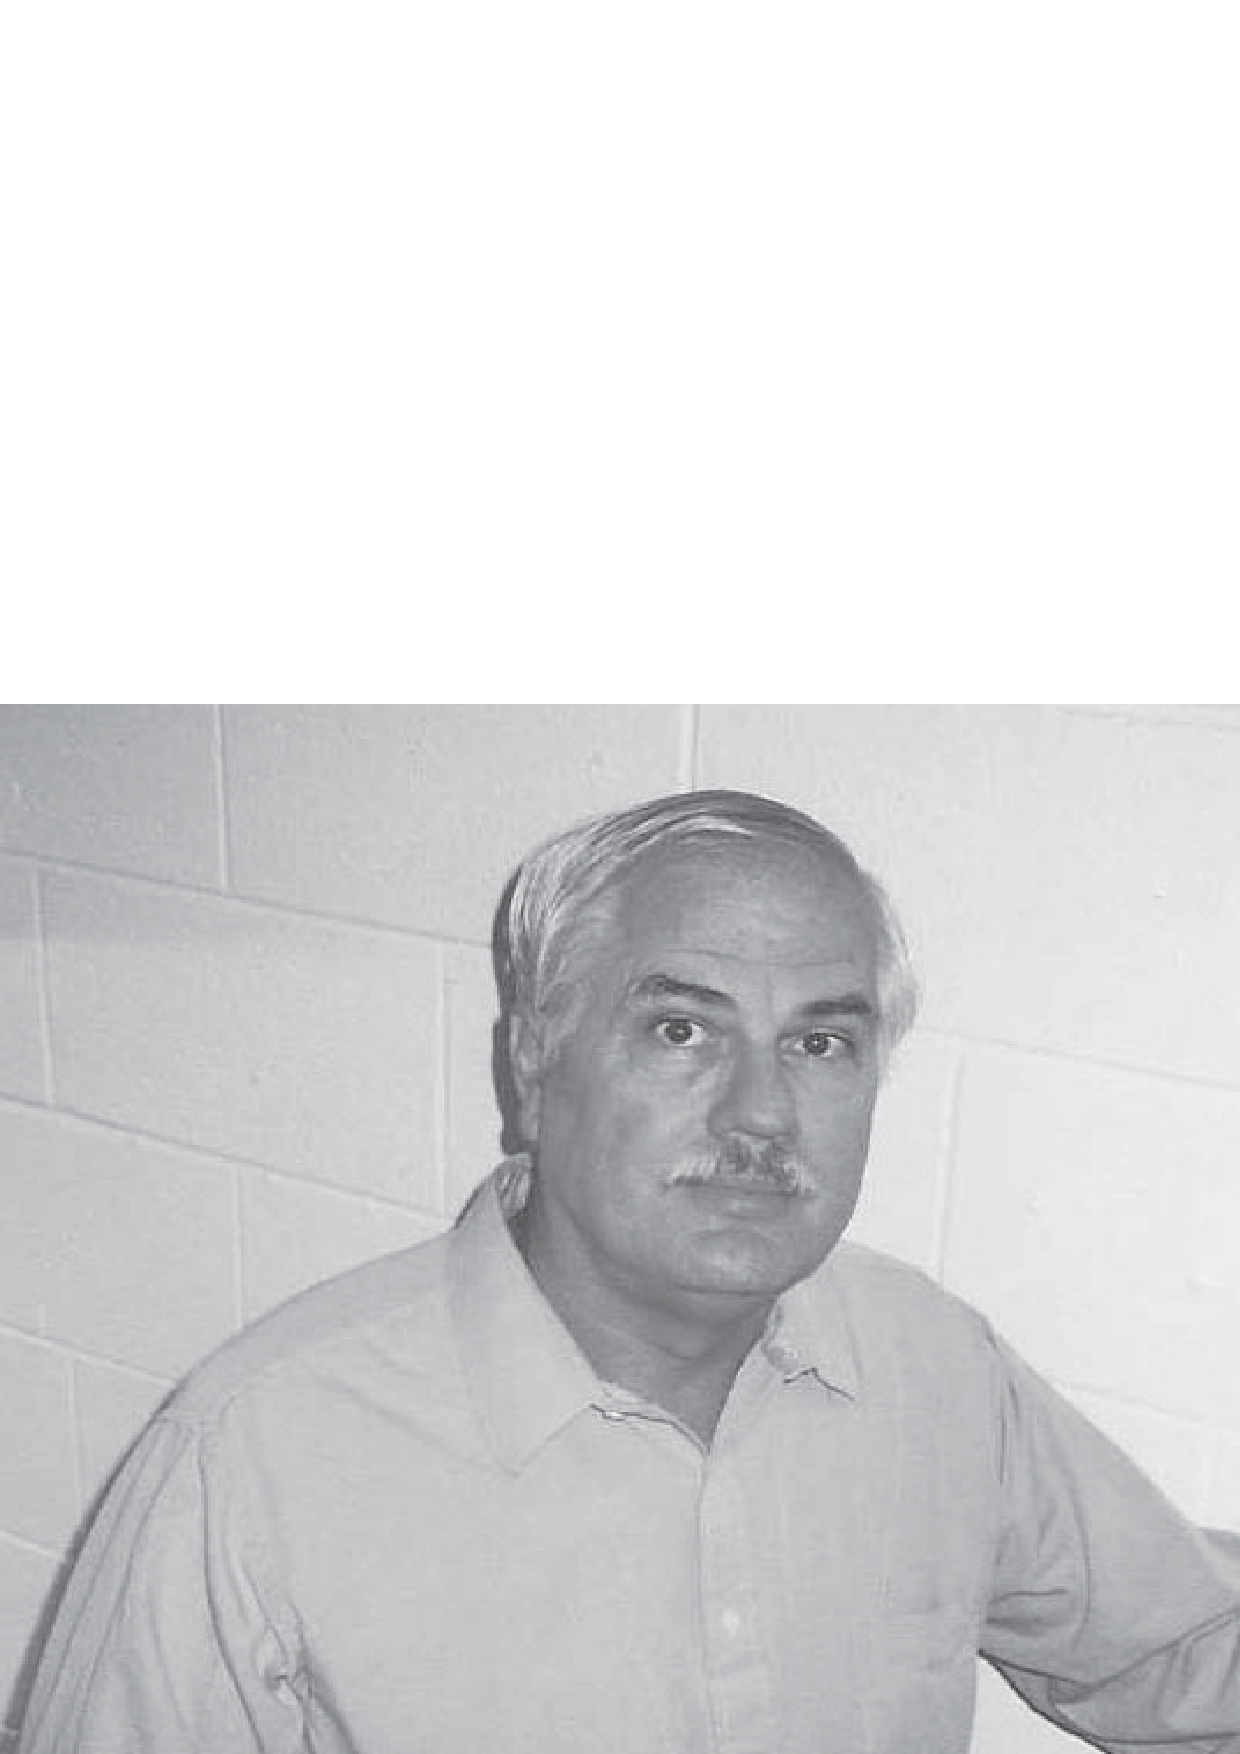
\includegraphics{dpsweb}}
\end{center}

\newpage

\begin{thebibliography}{[1]}\label{references}
\addcontentsline{toc}{section}{\protect\numberline{}References}
%\backrefparscanfalse
\let\backrefprint\relax
\def\srtln{\vskip-\baselineskip\vskip-\parsep}
\def\lngln{\vskip-\parsep}

\bibitem{webpage:XFASpec}\hypertarget{references}{}%
Adobe XML Forms Architecture (XFA) Specification, Version 3.3, Adobe Systems, Inc.,
Jan.\ 2012\backrefprint
   \lngln\hfill{\small\url{partners.adobe.com/public/developer/xml/index_arch.html}}

\bibitem{webpage:CSS2}
Cascading Style Sheets (CSS 2.2) Specification, Editors: Bert Bos \textsl{et al.},
World Wide Web Consortium (W3C), June 2011
   \lngln\hfill{\small\url{https://www.w3.org/TR/CSS2/}}

\bibitem{tech:AcroJS}
   JavaScript for Acrobat API Reference,
   Adobe Systems, Inc., May 2015
   \lngln\hfill{\small\url{adobe.com/devnet/acrobat/documentation.html}}

\bibitem{book:pdfspec}
    PDF Reference, Sixth Edition, Version 1.7, Adobe Systems, Inc., 2006
    \lngln\hfill{\small\url{adobe.com/devnet/pdf/pdf_reference_archive.html}}


\end{thebibliography}



% Adobe XML Forms Architecture (XFA) Specification, version 3.3, Jan. 2012,
% http://partners.adobe.com/public/developer/xml/index_arch.html

\end{document}

\bVerb\takeMeasure{\string\useNoHints\quad\string\useHints}%
\begin{dCmd}[commandchars=!()]{\bxSize}
\useNoHints!quad\useHints
\end{dCmd}
\eVerb The commands are used between \env{card} environments to change the
default usage of hints. When hints are \emph{not provided}, a simple message
defined by the command \cs{noHintProvided} (see \autopageref{noHintProvided}) appears on the hint page.
